% Introduction

\chapter{Introduction}
% \addcontentsline{toc}{chapter}{Introduction}  % if not numbered chapter

\label{Introduction} % For referencing the chapter elsewhere, use \Cref{Introduction}

%----------------------------------------------------------------------------------------

Some paragraph of text here.
To be dispatched in relevant places:

\begin{figure}[h]
  \centering
  \includegraphics*[width=0.5\columnwidth]{Figures/placeholder.png}
  \caption{The CERN Accelerator Complex as of 2020. This graphic indicates the first year of operation for each accelerator, as well as its circumference. Not to scale.}
  \label{fig:cern_accelerator_complex}
\end{figure}


\begin{figure}[h]
  \centering
  \includegraphics*[width=0.5\columnwidth]{Figures/placeholder.png}
  \caption{Cross-section of an LHC superconducting dipole magnet (see https://cds.cern.ch/record/40524).}
  \label{fig:lhc_dipole_crosssection}
\end{figure}


\begin{figure}[h]
  \centering
  \includegraphics*[width=0.5\columnwidth]{Figures/placeholder.png}
  \caption{The LHC ring with the purpose of the main sections. Not to scale.}
  \label{fig:lhc_ring_sections}
\end{figure}

As mentioned, each Insertion Region is separated from the previous one by an arc and has its own purpose:
\begin{enumerate}
    \item IR1 houses the ATLAS experiment
    \item IR2 houses the ALICE experiment and the injection of Beam1
    \item IR3 houses the off-momentum collimation cleaning (ref https://accelconf.web.cern.ch/ipac2016/doi/JACoW-IPAC2016-WEPMW007.html)
    \item IR4 houses the RF cavities to accelerate the beams
    \item IR5 houses the CMS experiment
    \item IR6 houses the beams' extraction to the dumps (ref https://cds.cern.ch/record/1392619)
    \item IR7 houses the betatronic collimation cleaning (ref https://cds.cern.ch/record/1056681)
    \item IR8 houses the LHCb experiment and the injection of Beam2
\end{enumerate}

\begin{figure}[h]
  \centering
  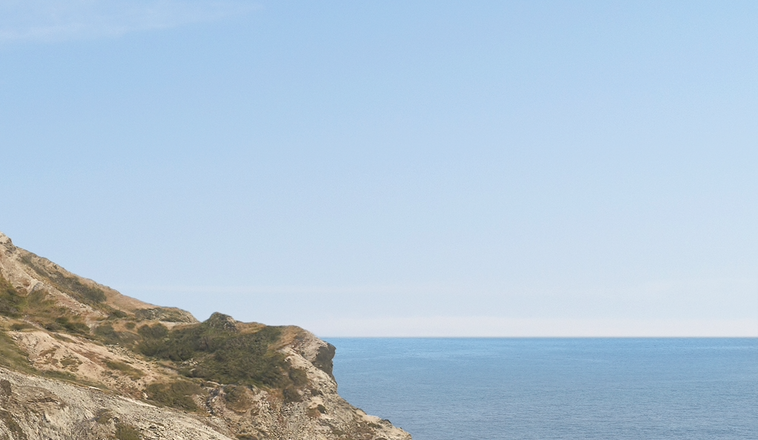
\includegraphics[width=0.5\columnwidth]{Figures/placeholder.png}
  \caption{Integrated luminosity in the four experiments of the LHC during the 2017-2018 LHC Run 2.}
  \label{fig:run_II_luminosities}
\end{figure}


% \begin{tabular}{lcc}
% \hline Parameters & Nominal LHC (design) & HL-LHC (standard) \\
% \hline Energy [TeV] & 7 & 7 \\
% Bunch spacing (ns) & 25 & 25 \\
% Nb. of bunches & 2808 & 2760 \\
% Nb. of collisions (IP1/IP5) & 2808 & 2748 \\
% Bunch charge [$10^{11}$] & 1.15 & 2.2 \\
% Total current [A] & 0.58 & 1.11 \\
% \hline
% $\beta^{*}$~[cm] & 55 & 15 \\
% Crossing angle [$\mu$ rad] & 285 & 500 \\
% Beam separation [$\sigma$] & 9.4 & 10.5 \\
% Norm. transverse emittance $[\mu m.rad]$ & $3.75$ & $2.5$ \\
% \hline Peak luminosity (w/o crab cavities) [$10^{34}$ ~Hz / $cm^{-2}$] & 1.0 & 8.1 \\
% Leveled luminosity $\left[10^{34} \mathrm{~Hz} / \mathrm{cm}^{-2}\right]$ & $\mathrm{NA}$ & 5.0 \\
% Leveling time [h] & $\mathrm{NA}$ & $7.2$ \\
% \hline
% \caption{Comparison of the LHC and HL-LHC baseline parameters.}
% \label{lhc_vs_hllhc_parameters}
% \end{tabular}

\begin{figure}[h]
  \centering
  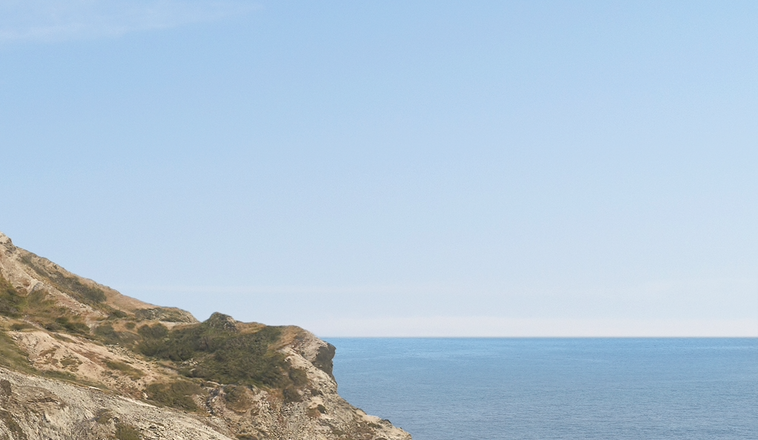
\includegraphics[width=0.5\columnwidth]{Figures/placeholder.png}
  \caption{Beam positions around the two high luminosity Interaction Points during the 2018 LHC Run. The dipoles are represented by blue rectangles while the quadrupoles by red ones.}
  \label{fig:ir1_ir5_beam_positions}
\end{figure}

%----------------------------------------------------------------------------------------

\section{Motivations}

\section{Thesis Outline}

\section{The CERN Accelerator Complex and its Upgrade}

\subsection{An Overview of CERN History}

\subsection{The Large Hadron Collider and its Injectors}

\subsection{The Concept of Luminosity}

\subsection{The LHC Performance and the HL-LHC Upgrade}
